\chapter{Marco teórico: Autómatas celulares neuronales}

En los últimos años, los autómatas celulares neuronales surgieron como una extensión de los clásicos, con las capacidades de aprendizaje y generalización propias de las redes neuronales artificiales. Esta integración permite que la regla de transición, tradicionalmente fija, sea parametrizable y entrenable mediante técnicas de aprendizaje supervisado.

Las primeras aproximaciones copiaban el funcionamiento de un autómata celular usando una red neuronal convolucional \cite{gilpinNCA}. Este método fue dado a conocer por Mordvintsev y otros \cite{mordvintsevNCA}, quienes entrenaron un modelo que aprende de dinámicas locales a partir de ejemplos. Como resultado, las interacciones locales básicas cumplen un objetivo en específico, mostrando propiedades de crecimiento, regeneración, autoorganización y morfogénesis.

Los autómatas celulares neuronales son entonces un tipo de autómatas celulares, pero cuya función de transición está definida como una red neuronal artificial. Retomando las definiciones previas, podemos decir entonces que:

\begin{definition}
	
	Un autómata celular es neuronal si la regla local $\mathcal{R}$ está dada como:
	
	\[
	\mathcal{R} = F_\theta: \mathbb{R}^{|\mathcal{N}|} \to \mathbb{R}^1
	\]
	
	donde:
	
	\begin{itemize}
		
		\item $F_\theta$ es una red neuronal parametrizada por $\theta$.
		
		\item $ \theta = \{ w_{uv}, b_v : (u, v) \in E, v \in V \}$ es el conjunto de parámetros entrenables.
		
		\item $\mathbb{R}^{|\mathcal{N}|}$ corresponde al espacio de entrada definido por la vecindad $\mathcal{N}$.
		
		\item $\mathbb{R}^1$ define el valor de salida que representa el nuevo estado de la célula central.
		
	\end{itemize}
	
\end{definition}

La figura \ref{fig:nca} muestra la relación existente entre estas dos tecnologías. En el paso $N$ se tiene una configuración bidimensional con vecindad de Neumann. El estado de cada elemento dentro de la vecindad funciona como valor de entrada para la red neuronal entrenada y devuelve un único resultado. Este resultado corresponde a la salida de la célula central, es decir, a la cual se le está aplicando.

\begin{figure}[H]
	
	\centering
	
	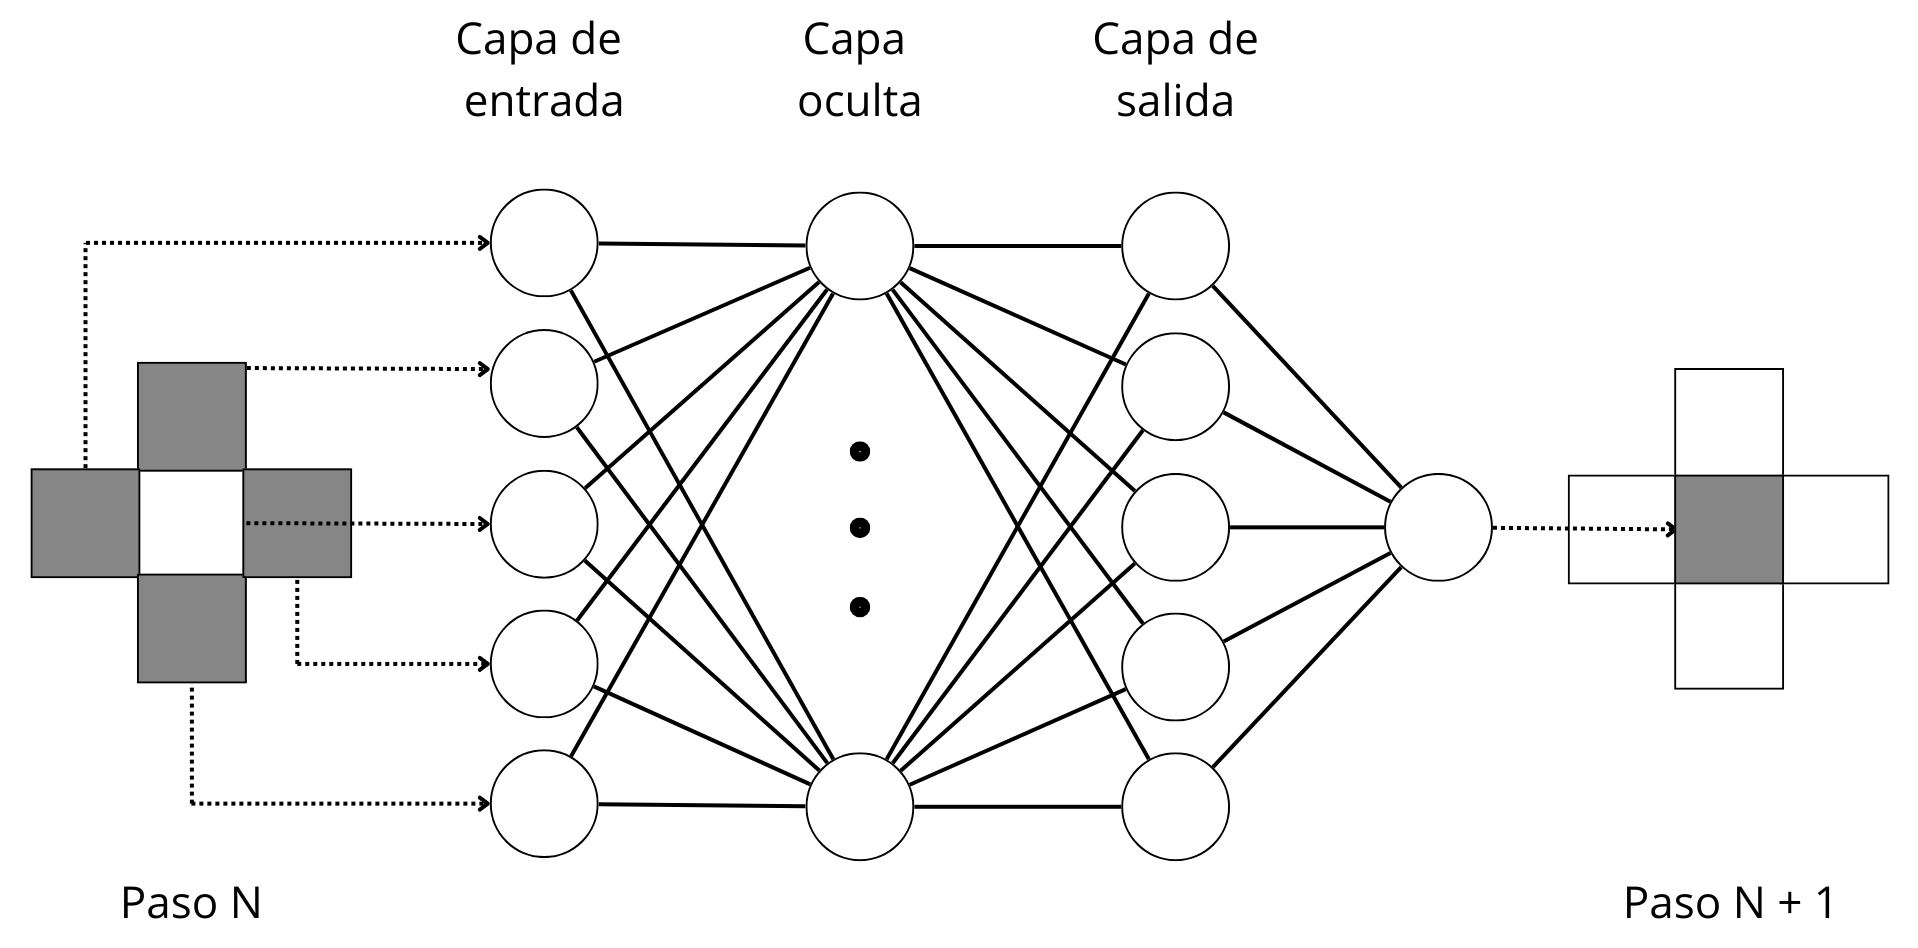
\includegraphics[width=0.8\textwidth]{img/NCA.png}
	
	\caption{Representación gráfica de la red neuronal.}
	
	\label{fig:nca}
	
\end{figure}

Cada célula aplica una misma red neuronal local $F_\theta$ sobre su vecindad inmediata. La entrada de la red consiste en los estados de las celdas dentro de la vecindad y la salida es el nuevo estado de la célula central. 

$F_\theta$ suele representarse como una red neuronal artificial convolucional que permite procesar localmente la información espacial preservando la estructura $D$-dimensional. 

A diferencia de los autómatas clásicos, donde las reglas son explícitas y definidas manualmente, los autómatas celulares neuronales aprenden sus reglas mediante un proceso de entrenamiento. Se establece un grupo de condiciones iniciales $X_0$ y un estado final $X^*$. Luego, la red $F_\theta$ se ajusta para reducir una función de pérdida $\mathcal{L}(X_T, X^*)$, que mide la diferencia entre la configuración obtenida después de $T$ pasos y el estado deseado. Este proceso puede expresarse como:

\[
\theta^* = \arg\min_\theta \mathcal{L}(F_\theta^{(T)}(X_0), X^*).
\]

Durante el entrenamiento, se emplean técnicas de retropropagación a través del tiempo y optimización por gradiente descendente. Esto permite que la red aprenda comportamientos dinámicos complejos, tales como el crecimiento morfológico, la regeneración parcial o la adaptación frente a perturbaciones.

Como se muestra a continuación, esta herramienta ha demostrado ser capaz de generar patrones autoorganizados y adaptativos sin necesidad de una programación explícita de reglas. Algunos ejemplos incluyen:

\begin{itemize}
	
	\item \textbf{Morfogénesis:} Crecimiento de formas y estructuras similares a organismos biológicos.
	
	\item \textbf{Regeneración:} Capacidad de reconstruir regiones dañadas o eliminadas de la configuración.
	
	\item \textbf{Modelado de sistemas complejos:} Simulación de fenómenos físicos, ecológicos o sociales mediante interacciones locales entrenables.
	
\end{itemize}

Esta mezcla de comportamiento que aparece por sí mismo y la habilidad de aprender hace que los autómatas celulares neuronales sean una herramienta muy útil para estudiar sistemas que se organizan solos y que se adaptan.

En el transcurso de este marco teórico se abordaron los conceptos fundamentales que sustentan y contextualizan la presente investigación, tales como los sistemas complejos, los autómatas celulares, las redes neuronales y los autómatas celulares neuronales. Estos elementos permiten comprender los principios que rigen la dinámica de sistemas con comportamiento emergente y las herramientas computacionales que posibilitan su modelado y simulación.

La integración de estos fundamentos teóricos proporciona una base sólida para el diseño, desarrollo y validación del simulador propuesto. En particular, la comprensión de la relación entre las reglas locales y los comportamientos globales de los autómatas celulares, junto con la capacidad de aprendizaje de las redes neuronales, constituye el punto de partida. Esto es crucial para la implementación de autómatas celulares neuronales capaces de adaptarse y evolucionar dentro de entornos complejos.

Así, el marco teórico no solo establece el contexto conceptual del trabajo, sino que también apoya las decisiones técnicas y metodológicas que ayudarán a crear un modelo de simulación que sea flexible, escalable y que esté alineado con los objetivos de la investigación.

\clearpage